\documentclass[12pt]{article}
\usepackage{fullpage}
\usepackage{titlesec}
\usepackage{tikz}
\usepackage{amsfonts,amssymb}
\usepackage{amsmath}
\usepackage{comment}
\usetikzlibrary{automata, positioning}

\input ../libraries/mac.tex
\input ../libraries/mathmac.tex

\begin{document}
\pagestyle{plain}
\titleformat{\subsection}[runin]
  {\normalfont\large\bfseries}{\thesubsection}{1em}{}

\title{Homework 4}
\author{Brooke Fugate, Michael O'Connor, Rohan Shah}
\date{}

\maketitle

\section*{Problem B6}
\subsection*{1}
\begin{center}
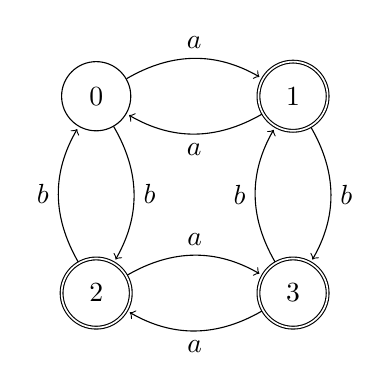
\begin{tikzpicture}[shorten >=1pt, node distance=2.5cm, on grid, auto]
  \node[state] (q0) {0};
  \node[state, accepting] (q1) [right=of q0] {1};
  \node[state, accepting] (q2) [below=of q0] {2};
  \node[state, accepting] (q3) [right =of q2] {3};
  \path[->]
(q0) edge [bend left] node {$a$} (q1)
(q0) edge [bend left] node {$b$} (q2)
(q1) edge [bend left] node {$a$} (q0)
(q1) edge [bend left] node {$b$} (q3)
(q2) edge [bend left] node {$a$} (q3)
(q2) edge [bend left] node {$b$} (q0)
(q3) edge [bend left] node {$a$} (q2)
(q3) edge [bend left] node {$b$} (q1)
  ;
\end{tikzpicture}
\end{center}

\subsection*{2}
$((ab+ba)(aa+bb)^*(ba+ab) + bb + aa)^* (a+b+(ab+ba)(aa+bb)^*(\epsilon + a + b))$

\end{document}
